\documentclass[11pt,a4paper]{article}
\usepackage[T1]{fontenc}
\usepackage[margin=2.3cm]{geometry}
\usepackage{amsmath,amssymb}
\usepackage{graphicx}
\usepackage[dvipsnames]{xcolor}
\usepackage{enumitem}
\usepackage[colorlinks=true,linkcolor=blue,urlcolor=blue]{hyperref}
\setlength{\parskip}{0.6em}
\setlength{\parindent}{0pt}
\begin{document}

\begin{center}{\LARGE\bfseries openepidemic}\\[0.4em]{\large Fit an outbreak model to noisy data and test vaccination, in three sessions.}\\[0.2em]\small PAN IIT OSS explainer \textbullet{} secondary school to diploma / undergraduate (levels 3-5)\end{center}

\section*{Why this exists}
Outbreak models turn the simple idea that an infection spreads when each case infects more than one other into equations that can be solved and fitted. This explainer shows the mathematics with invented data, so you can build it yourself. It is general education: the models are teaching tools, not forecasts, not medical advice and not a basis for public-health decisions.

\section*{The end goal}
Fit an SIR model to outbreak data and test vaccination (general education only). The end goal is to fit an SIR model to outbreak data and to test vaccination in a synthetic town: solving the equations, estimating beta and gamma with honest uncertainty, and understanding what the data can and cannot tell. The same ideas of fitting and identifiability are used across science.

\section*{How the three sessions build up}
\begin{enumerate}[nosep]
\item \textbf{Session 1: Three boxes with arrows: how an outbreak rises and falls} (Level 1, conceptual interactive model, 60 min).
\item \textbf{Session 2: The SIR equations, R0 and herd immunity} (Level 2, mathematical engineering model, 75 min).
\item \textbf{Session 3: Simulate, fit and test: SIR with data, chance and vaccination} (Level 3, simulation and validation, 90 min).
\end{enumerate}

\section{Session 1: Three boxes with arrows: how an outbreak rises and falls}

\subsection*{A. Real-world problem}
GENERAL EDUCATION ONLY: this is a toy with invented people. It is not a forecast, not medical advice and not a basis for public-health decisions. When a new infection reaches a town, why does one outbreak explode while another fizzles out? And why does the number of sick people rise, reach a peak, and then fall even though nobody did anything special at the peak? Modellers sort people into three boxes: Susceptible (could catch it), Infected (have it and can pass it on) and Recovered (had it, now immune). Two arrows move people: infection (S to I) and recovery (I to R).

\subsection*{B. Concept and theory}
In a small time step dt (days), the number of new infections is beta times S times I divided by N times dt: it is large when many people are susceptible and many are infectious, because that is when meetings between the two are common. The number of new recoveries is gamma times I times dt: a fixed share of the infected people recovers each day. People only move, so S + I + R = N always. One infected person stays infectious for about 1/gamma days and infects people at rate beta, so infects about beta / gamma others when nearly everybody is susceptible. This number is R0. If R0 is above 1 each case replaces itself with more than one case and the outbreak grows; if it is below 1 the outbreak dies away. The curve of infected people peaks later, when so many people have already recovered that the infected can no longer find enough susceptible people to pass the infection on.

\begin{itemize}[nosep]
\item S, I, R: numbers of susceptible, infected and recovered people (people)
\item N: total number of people (S + I + R) (people)
\item beta: contact rate: infections caused per infected person per day when everyone is susceptible (1/day)
\item gamma: recovery rate = 1 / (days a person is infectious) (1/day)
\item R0: basic reproduction number = beta / gamma (no unit)
\item dt: time step (days)
\end{itemize}

\begin{equation*}
\text{new infections}=\beta\,\dfrac{S\,I}{N}\,\Delta t,\qquad \text{new recoveries}=\gamma\,I\,\Delta t
\end{equation*}

\begin{equation*}
S+I+R=N\quad\text{(people only move between boxes)}
\end{equation*}

\begin{equation*}
R_0=\dfrac{\beta}{\gamma}\quad\text{(people infected by one case in a fully susceptible town)}
\end{equation*}

\begin{center}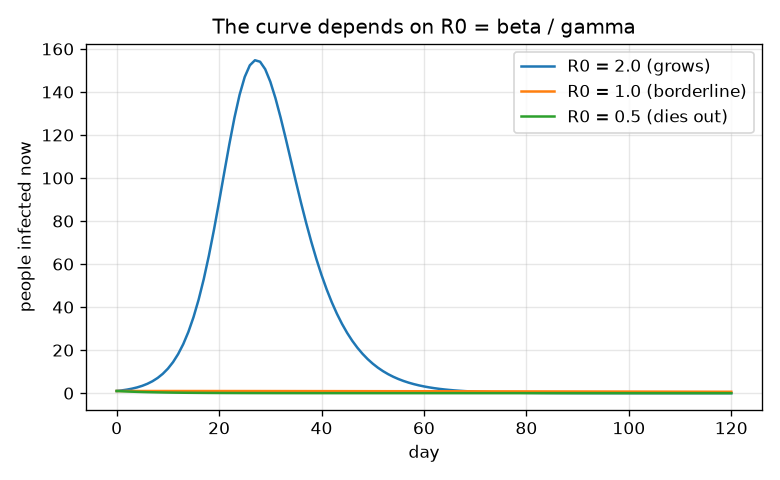
\includegraphics[width=0.85\linewidth]{figures/s01_r0_compare.png}\\\small Infected people for R0 = 2, 1 and 0.5: only R0 above 1 gives an outbreak.\end{center}

\subsection*{E. Worked example}
A town has N = 1000 people, 999 susceptible and 1 infected. With beta = 0.5 and gamma = 0.25 per day, move the people for one day (dt = 1) and find R0.
\begin{enumerate}[nosep]
\item New infections = 0.5 * 999 * 1 / 1000 * 1 = 0.4995 people.
\item New recoveries = 0.25 * 1 * 1 = 0.25 people.
\item S = 999 - 0.4995 = 998.5005; I = 1 + 0.4995 - 0.25 = 1.2495; R = 0 + 0.25 = 0.25.
\item Check: 998.5005 + 1.2495 + 0.25 = 1000, so nobody was lost.
\item R0 = beta / gamma = 0.5 / 0.25 = 2, so one case infects about 2 others: 1, 2, 4, 8 cases over four generations.
\end{enumerate}
\textbf{Answer.} After one day S = 998.5005, I = 1.2495, R = 0.25, and R0 = 2. (With the finer 0.1 day steps used in lesson.py the town on day 10 has S = 978.0, I = 11.4, R = 10.6.)

\subsection*{F. Questions}
\begin{enumerate}[nosep]
\item \textbf{Conceptual.} Why does the number of infected people fall after the peak even if nobody changes their behaviour?
\item \textbf{Numerical.} A town has beta = 0.3 and gamma = 0.1 per day. Find R0 and the number of cases in generation 3, starting from one case.
\item \textbf{Graph and simulation interpretation.} In the S, I, R figure, on which day is the peak, roughly how many people are infected then, and what happens to R at that moment?
\item \textbf{Design and optimisation challenge.} Design: with gamma = 0.25 per day, the town's contact rate is beta = 0.5. A school-closure plan could reduce beta. What beta makes R0 equal to exactly 1, and what happens if the plan reaches beta = 0.2? State one reason your answer might be too optimistic.
\end{enumerate}

\section{Session 2: The SIR equations, R0 and herd immunity}

\subsection*{A. Real-world problem}
GENERAL EDUCATION ONLY: teaching model, invented numbers; not a forecast, not medical advice, not a basis for public-health decisions. Before any outbreak, a town can ask two questions of a simple model: how many people would be infected in total if nothing were done, and what share of the town must already be protected so that an infection cannot take off? The first is the final size, the second the herd immunity threshold. Both follow from the SIR equations and one number, R0.

\subsection*{B. Concept and theory}
Turn the boxes of Session 1 into rates of change. People leave S at the rate beta S I / N, the same people enter I, and I loses gamma I people to R. Because S + I + R = N, the three equations add to zero. The infected number grows when dI/dt is positive, that is when beta S / N is above gamma, which is R0 S / N above 1. At the start S is close to N, so growth needs R0 above 1. The effective reproduction number R\_eff = R0 S / N falls as S falls; at the peak R\_eff = 1. Herd immunity: if a fraction p of the town is protected at the start, R\_eff = R0 (1 - p), which is below 1 when p is above 1 - 1/R0. Final size: dividing dS/dt by dR/dt gives dS/dR = -R0 S / N, so S = S0 exp(-R0 R / N); at the end I = 0, so with z the fraction ever infected and S0 close to N, 1 - z = exp(-R0 z). This equation has no closed-form solution, so we solve it with Newton's method. Design: a vaccine with efficacy e protects a fraction e of those vaccinated; with coverage v the protected share is v e, so we need v above (1 - 1/R0) / e. If e is below 1 - 1/R0 this exceeds 100 percent and vaccination alone cannot stop the spread. For an imperfect (leaky) vaccine the same count holds on average: some vaccinated people stay susceptible, so more people must be vaccinated.

\begin{itemize}[nosep]
\item beta: contact rate (1/day)
\item gamma: recovery rate (1/day)
\item R0: beta / gamma (no unit)
\item R\_eff: R0 times the susceptible share S / N (no unit)
\item z: fraction of the town ever infected (final size) (no unit)
\item v: vaccination coverage (share vaccinated) (no unit (0 to 1))
\item e: vaccine efficacy: share of the vaccinated who are protected (no unit (0 to 1))
\item N: population (people)
\end{itemize}

\begin{equation*}
\dfrac{dS}{dt}=-\beta\dfrac{S I}{N},\qquad \dfrac{dI}{dt}=\beta\dfrac{S I}{N}-\gamma I,\qquad \dfrac{dR}{dt}=\gamma I
\end{equation*}

\begin{equation*}
R_0=\dfrac{\beta}{\gamma},\qquad \dfrac{dI}{dt}>0\iff R_0\dfrac{S}{N}>1
\end{equation*}

\begin{equation*}
p_c=1-\dfrac{1}{R_0}\quad\text{(herd immunity threshold)}
\end{equation*}

\begin{equation*}
z=1-e^{-R_0 z}\quad\text{(final size, } S_0\approx N\text{)}
\end{equation*}

\begin{equation*}
v>\dfrac{1-1/R_0}{e}\quad\text{(coverage needed with efficacy } e\text{)}
\end{equation*}

\begin{equation*}
\dfrac{I_{\max}}{N}\approx 1-\dfrac{1+\ln R_0}{R_0}
\end{equation*}

\begin{center}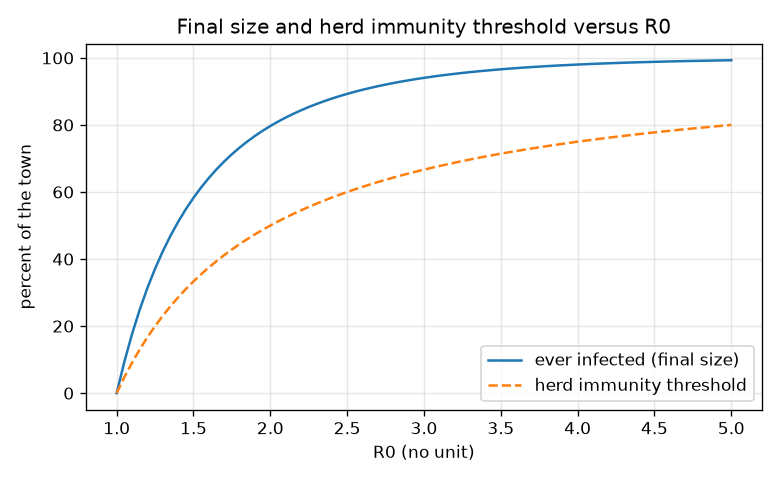
\includegraphics[width=0.85\linewidth]{figures/s02_final_size.png}\\\small Final size and herd immunity threshold against R0.\end{center}

\subsection*{E. Worked example}
(a) For R0 = 3 find the herd immunity threshold. (b) For R0 = 2 check that z = 0.797 is the final size. (c) Find the coverage needed for R0 = 3 when the vaccine efficacy is 0.9.
\begin{enumerate}[nosep]
\item (a) p\_c = 1 - 1/3 = 0.667, that is 66.7 percent of the town.
\item (b) Evaluate the right-hand side at z = 0.797: 1 - exp(-2 * 0.797) = 1 - exp(-1.594) = 1 - 0.203 = 0.797. The two sides agree, so z = 0.797: about 79.7 percent of the town is ever infected.
\item (c) v \textgreater{} 0.667 / 0.9 = 0.741, that is 74.1 percent.
\item Check (c): protected share = 0.741 * 0.9 = 0.667; R\_eff = 3 * (1 - 0.667) = 1.
\end{enumerate}
\textbf{Answer.} (a) 66.7 percent. (b) about 79.7 percent are ever infected. (c) 74.1 percent coverage. Imperfect protection raises the coverage needed from 66.7 to 74.1 percent; with efficacy 0.6 it would be 111 percent, which is impossible.

\subsection*{F. Questions}
\begin{enumerate}[nosep]
\item \textbf{Conceptual.} Explain in words why the herd immunity threshold is 1 - 1/R0 and why a larger R0 needs a larger share protected.
\item \textbf{Numerical.} R0 = 4. Find the herd immunity threshold. With a vaccine of efficacy 0.8, what coverage is needed?
\item \textbf{Graph and simulation interpretation.} In the vaccination figure, how do the peak height and peak day change as coverage goes from 0 to 30 to 50 percent? What does this tell you about R\_eff?
\item \textbf{Design and optimisation challenge.} Design: for R0 = 3 the town can only buy a vaccine with efficacy 0.6. Is vaccination alone enough to stop the infection spreading? What combination of measures could work, and what assumption does your answer rely on?
\end{enumerate}

\section{Session 3: Simulate, fit and test: SIR with data, chance and vaccination}

\subsection*{A. Real-world problem}
GENERAL EDUCATION ONLY: every data set in this session is invented. The model is a teaching tool, not a forecast, not medical advice and not a basis for public-health decisions. Case counts arrive as noisy daily numbers. A modeller asks: which contact rate beta and recovery rate gamma reproduce them, how sure are we, and what would vaccinating part of the town first do to the peak? Two traps wait: data from before the peak hardly constrain the answer, and reporting delays shift the whole picture. And one more surprise: with a single starting case, an outbreak can simply die out by luck.

\subsection*{B. Concept and theory}
Numerical solution: RK4 advances (S, I, R) over a step h using four slopes k1 to k4 and the weighted average (k1 + 2 k2 + 2 k3 + k4) / 6; its error falls with the fourth power of h. We validate it against three trusted results: S + I + R = N, the final size equation z = 1 - exp(-R0 z), and the early exponential growth I \textasciitilde{} exp(r t) with r = gamma (R0 - 1) (found by linearising dI/dt for S close to N). Synthetic data: the expected number of new infections on day k is S(k) - S(k+1); each day's reported count is a Poisson random number with that mean. Fitting: least squares chooses (beta, gamma) to minimise the sum of squared differences between model and data. We use a grid search and then Gauss-Newton, which linearises the model with its Jacobian matrix J and gives the covariance of the estimates, s\textasciicircum{}2 (J\textasciicircum{}T J)\textasciicircum{}(-1). Because many data sets from the same truth give a spread of estimates, repeating the experiment measures the uncertainty. Identifiability: early on the data are mostly exponential growth, which fixes the difference beta - gamma but not beta and gamma separately, so the two estimates move together (correlation near 1). Chance: the Gillespie method draws random waiting times, with infection events at rate beta S I / N and recovery events at rate gamma I. For one starting case in a large town the number of cases early on behaves as a branching process whose extinction probability is gamma / beta = 1/R0. Vaccination before the outbreak moves v e N people from S to R.

\begin{itemize}[nosep]
\item h: RK4 step size (days)
\item r: early exponential growth rate = gamma (R0 - 1) (1/day)
\item J: Jacobian: derivative of model daily cases with respect to beta and gamma (people/day per (1/day))
\item s\textasciicircum{}2: residual variance of the fit (people\textasciicircum{}2/day\textasciicircum{}2)
\item P\_ext: probability that an outbreak from one case dies out (no unit)
\item v, e: coverage and efficacy (no unit)
\item peak: largest number infected at once (people)
\end{itemize}

\begin{equation*}
\mathbf y_{n+1}=\mathbf y_n+\dfrac{h}{6}\left(\mathbf k_1+2\mathbf k_2+2\mathbf k_3+\mathbf k_4\right)
\end{equation*}

\begin{equation*}
I(t)\approx I_0\,e^{r t},\qquad r=\gamma(R_0-1)=\beta-\gamma
\end{equation*}

\begin{equation*}
\min_{\beta,\gamma}\ \sum_k\left(c_k-m_k(\beta,\gamma)\right)^2,\qquad \Delta\theta=\left(J^{\mathsf T}J\right)^{-1}J^{\mathsf T}(c-m),\qquad \mathrm{Cov}\approx s^2\left(J^{\mathsf T}J\right)^{-1}
\end{equation*}

\begin{equation*}
P_{\mathrm{ext}}\approx \dfrac{1}{R_0}=\dfrac{\gamma}{\beta}\quad\text{(one starting case, large town, } R_0>1\text{)}
\end{equation*}

\begin{equation*}
R_{\mathrm{eff}}=R_0\,(1-v\,e)
\end{equation*}

\begin{center}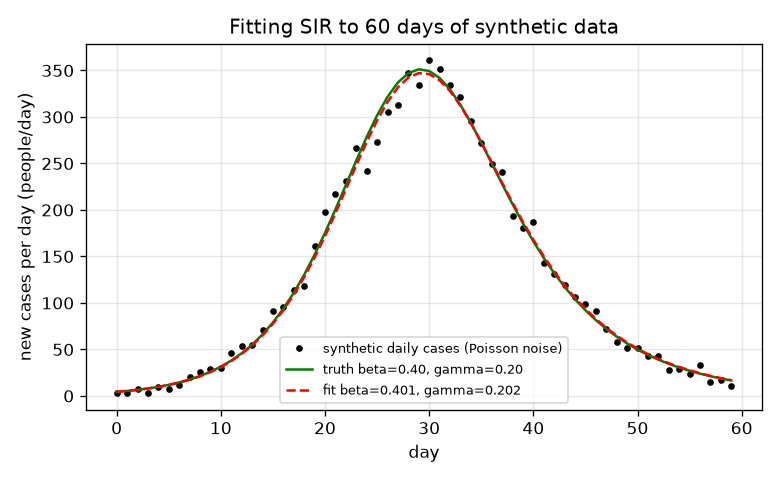
\includegraphics[width=0.85\linewidth]{figures/s03_fit_full.png}\\\small Synthetic noisy daily cases, the true curve and the fitted curve over 60 days.\end{center}

\subsection*{E. Worked example}
A synthetic town of 50000 people has 10 infected people, beta = 0.4, gamma = 0.2 per day and a vaccine with efficacy 0.9. Its hospital line is 3000 people infected at once. Find the smallest whole-percent coverage that keeps the peak under the line.
\begin{enumerate}[nosep]
\item R0 = 0.4 / 0.2 = 2. Without vaccination the RK4 simulation gives a peak of 7676 people, far over the line.
\item Protected share = coverage * 0.9. At 23 percent coverage the protected share is 20.7 percent: R\_eff = 2 * (1 - 0.207) = 1.59 and the simulated peak is 3125 people, still over the line.
\item At 24 percent coverage the protected share is 21.6 percent: R\_eff = 1.57 and the peak is 2961 people, under the line.
\item Note that R\_eff is far above 1 in both cases: the line is kept not by stopping the outbreak but by flattening it.
\end{enumerate}
\textbf{Answer.} The smallest passing coverage is 24 percent (peak 2961 people); 23 percent fails (3125). Sensitivity: with beta 10 percent lower (0.36) the answer is 17 percent, with beta 10 percent higher (0.44) it is 31 percent, and a vaccine with efficacy 0.6 needs 36 percent. A 10 percent error in beta moves the answer a lot, so a real plan would need a large margin; this is a classroom exercise only.

\subsection*{F. Questions}
\begin{enumerate}[nosep]
\item \textbf{Conceptual.} Why can the first two weeks of data fix the growth rate beta - gamma well but not beta and gamma separately?
\item \textbf{Numerical.} A fit to the first 14 days of the seed-1000 data gives beta = 0.477 and gamma = 0.288. Compute R0 and beta - gamma, and compare both with the truth (beta 0.4, gamma 0.2).
\item \textbf{Graph and simulation interpretation.} In Figure 2, compare the left panel (14 days) and the right panel (60 days). What does the diagonal shape mean, and what should a modeller conclude from it?
\item \textbf{Design and optimisation challenge.} Design: the hospital line is 1000 people for the synthetic town of the worked example (efficacy 0.9, beta 0.4, gamma 0.2). Find the smallest coverage, then say what margin you would add if beta is uncertain by 10 percent, and state one trade-off.
\end{enumerate}

\section{Real-world mini-project}
\textbf{Keep a synthetic town under its hospital line.} GENERAL EDUCATION ONLY: the town is invented and the answer is a classroom exercise, never advice for a real place. A synthetic town of 50000 people has 10 infected people, beta = 0.4 and gamma = 0.2 per day (R0 = 2), and a vaccine with efficacy 0.9. Its hospital line is 3000 people infected at once. Use \texttt{peak\_with\_vaccination} and \texttt{min\_coverage\_for\_peak} from Session 3 to find the smallest whole-percent coverage that keeps the peak under the line, then test how fragile your answer is.

\section{The path ahead}
\begin{enumerate}[nosep]
\item \textbf{Session 4: Add age groups.} A two-group SIR model (for example children and adults) with a 2 by 2 contact matrix and group-specific vaccination.
\item \textbf{Session 5: Add an exposed stage (SEIR).} An SEIR model with latent rate sigma, solved with your RK4.
\item \textbf{Session 6: Fit with a reporting delay and under-reporting.} A fit of beta, gamma, delay and reporting fraction to synthetic data that has a 5-day delay.
\item \textbf{Session 7: Honest uncertainty with a Bayesian fit.} A random-walk Metropolis sampler for beta and gamma with a Poisson likelihood.
\item \textbf{Session 8: Target: the animated fit band and vaccination slider.} A two-panel animation like the Target, built on your own fitting and RK4 code.
\end{enumerate}

\section{Answers and hints}

\subsection*{Session 1}
\begin{enumerate}[nosep]
\item \textbf{Conceptual.} Hint: Think about who is left for an infected person to meet. Solution: After the peak so many people have recovered (and are immune) that an infected person meets mostly recovered people, so each case infects fewer than one other. New infections drop below new recoveries, so I falls. The outbreak does not end because the infection runs out of time but because it runs out of susceptible people.
\item \textbf{Numerical.} Hint: R0 = beta / gamma; each generation multiplies the number of cases by R0. Solution: R0 = 0.3 / 0.1 = 3. Generations: 1, 3, 9, 27, so generation 3 has 27 cases. Sanity check: R0 above 1, so the numbers grow. Units: R0 has no unit; the cases are people.
\item \textbf{Graph and simulation interpretation.} Hint: Find the highest point of the I curve and look at the other curves above that day. Solution: The peak is on day 27 with about 155 infected people. At that moment S is falling and R is rising, but the I curve is flat for an instant because new infections equal new recoveries. After that day R keeps rising and I falls.
\item \textbf{Design and optimisation challenge.} Hint: R0 = beta / gamma, so beta = R0 * gamma. Solution: For R0 = 1 we need beta = 1 * 0.25 = 0.25 per day: halving beta. At beta = 0.2, R0 = 0.8 and the number of infected people falls from the first day. Too optimistic because beta is not a dial we can set: contacts differ between people and groups, the model assumes equal mixing, and a change in behaviour is itself uncertain. This is a classroom exercise, not advice.
\end{enumerate}

\subsection*{Session 2}
\begin{enumerate}[nosep]
\item \textbf{Conceptual.} Hint: Each case must infect fewer than one other person; what share of contacts must be with protected people? Solution: Each case meets people at random; a fraction p of them are protected and cannot be infected. So a case infects R0 (1 - p) people. The outbreak cannot grow when this is below 1, which gives 1 - p \textless{} 1/R0, i.e. p \textgreater{} 1 - 1/R0. A larger R0 means each case would infect more people, so a larger share of contacts must be blocked.
\item \textbf{Numerical.} Hint: p\_c = 1 - 1/R0 and v = p\_c / e. Solution: p\_c = 1 - 1/4 = 0.75, that is 75 percent. v = 0.75 / 0.8 = 0.9375, about 93.8 percent. Check: protected share 0.9375 * 0.8 = 0.75, R\_eff = 4 * 0.25 = 1. Units: shares have no unit; multiply by 100 for percent.
\item \textbf{Graph and simulation interpretation.} Hint: Compare the three curves; compute R\_eff = 2 (1 - 0.9 v) for each. Solution: The peak falls from 1543 to 415 to 33 people and arrives later. R\_eff at the start is 2, 1.46 and 1.10: still above 1, so the infection still grows, but slowly, and fewer susceptible people are available. Coverage below the threshold reduces and delays the peak; it does not remove the outbreak.
\item \textbf{Design and optimisation challenge.} Hint: Compute the coverage needed; if it is above 100 percent, what else must change? Solution: Needed coverage = 0.667 / 0.6 = 1.11, which is 111 percent, impossible: even vaccinating everyone protects only 60 percent, below the 66.7 percent threshold. So R\_eff stays above 1 (3 * 0.4 = 1.2). A second measure must also reduce beta (or R0) by at least a factor of 1.2: then the effective R0 would be 2.5 or lower and the threshold 60 percent, which full coverage just reaches. The answer relies on equal mixing, a perfect random vaccination and a fixed efficacy. This is a classroom exercise, not advice.
\end{enumerate}

\subsection*{Session 3}
\begin{enumerate}[nosep]
\item \textbf{Conceptual.} Hint: During the exponential phase I(t) is proportional to exp((beta - gamma) t). What do two different pairs with the same difference look like? Solution: In the early phase new cases grow like exp(r t) with r = beta - gamma, so the data mostly measure r. Pairs such as (0.4, 0.2) and (0.48, 0.29) give almost the same growth rate (0.20 and 0.19), so the curves are nearly identical for two weeks: the sum of squared differences between them over 14 days is only 40 people\textasciicircum{}2, well inside the noise (the Poisson variance of the 14 counts adds up to 296 people\textasciicircum{}2), whereas over 60 days it is 55941 people\textasciicircum{}2 and the pairs are easy to tell apart. The estimates move together (correlation near 1). The curves only differ later, near and after the peak, when gamma controls how fast people leave I and beta controls how fast S is used up.
\item \textbf{Numerical.} Hint: R0 = beta / gamma, growth rate = beta - gamma. Solution: R0 = 0.477 / 0.288 = 1.66 against the true 2.0: about 17 percent low. beta - gamma = 0.477 - 0.288 = 0.189 against the true 0.2: only 5.5 percent low. The growth rate is far better determined than R0, which is the identifiability problem in numbers. (The standard errors of that fit are 0.10 and 0.12.)
\item \textbf{Graph and simulation interpretation.} Hint: Look at the width of the cloud along and across the diagonal. Solution: The cloud on the left is long along the diagonal and thin across it: beta and gamma can both be much too high or much too low together, as long as their difference is about 0.2. The standard deviations of the estimates are 0.080 (beta) and 0.097 (gamma) but the standard deviation of beta - gamma is only 0.018. On the right (60 days) the cloud is a tiny blob (0.006). A modeller should not quote beta or R0 from early data without wide error bars, and should report the well-determined combination.
\item \textbf{Design and optimisation challenge.} Hint: Use min\_coverage\_for\_peak(1000), then repeat with beta = 0.44. Solution: The smallest passing coverage for the 1000 line is 39 percent. Because the answer for 3000 changes from 24 to 31 percent when beta is 10 percent higher, a margin of at least a few percentage points above the nominal answer is sensible; also the true efficacy is uncertain. Trade-off: more coverage costs more and cannot exceed 100 percent, while a smaller margin risks exceeding capacity. This is a classroom exercise; real decisions need expert, much more detailed analysis.
\end{enumerate}

\section{How to join}
Read \texttt{CONTRIBUTING.md} in the repository, then pick an issue labelled \texttt{good first issue}. Repository: \url{https://github.com/KrunalPanchal1995/openepidemic}

\end{document}
